%%%%%%%%%%%%%%%%%%%%%%%%%%%%%%%%%%%%%%%%%
% Dreuw & Deselaer's Poster
% LaTeX Template
% Version 1.0 (11/04/13)
%
% Created by:
% Philippe Dreuw and Thomas Deselaers
% http://www-i6.informatik.rwth-aachen.de/~dreuw/latexbeamerposter.php
%
% This template has been downloaded from:
% http://www.LaTeXTemplates.com
%
% Edited by: Manfred Brill
%
% License:
% CC BY-NC-SA 3.0 (http://creativecommons.org/licenses/by-nc-sa/3.0/)
%%%%%%%%%%%%%%%%%%%%%%%%%%%%%%%%%%%%%%%%%

% ----------------------------------------------------------------------------------------
%  Kopf- und Fusszeile werden in beamertheme16pd2.sty definiert!
% ----------------------------------------------------------------------------------------

%----------------------------------------------------------------------------------------
%   PACKAGES AND OTHER DOCUMENT CONFIGURATIONS
%----------------------------------------------------------------------------------------
\documentclass[final,hyperref={pdfpagelabels=false}]{beamer}

\usepackage{todo}

\usepackage{wrapfig}

\usepackage[orientation=portrait, size=a0, scale=1.2]{beamerposter}

\usetheme{I6pd2} % Use the I6pd2 theme supplied with this template

\usepackage[german]{babel}
%\usepackage[english]{babel} % English language/hyphenation

\usepackage{amsmath,amsthm,amssymb,latexsym}

%\usepackage{times}\usefonttheme{professionalfonts}  % Uncomment to use Times as the main font
%\usefonttheme[onlymath]{serif} % Uncomment to use a Serif font within math environments

\boldmath % Use bold for everything within the math environment

\usepackage{booktabs} % Top and bottom rules for tables

\usepackage{multicol}

\usepackage{caption}
\usepackage{subcaption}
\usepackage{hyperref}
\usepackage[misc]{ifsym}
\usepackage[export]{adjustbox}
\usepackage{fontawesome}

\newcommand{\imagePath}{./figures}

\graphicspath{{figures/}} % Location of the graphics files

\usecaptiontemplate{\small\structure{\insertcaptionname~\insertcaptionnumber: }\insertcaption}
 % A fix for figure numbering

%----------------------------------------------------------------------------------------
%   TITLE SECTION
%----------------------------------------------------------------------------------------

\title{\huge Visual$\:$Raytrace}

\author{Benedict S\"arota}



\institute{Fachbereich Informatik und Mikrosystemtechnik}
%----------------------------------------------------------------------------------------

\begin{document}

\addtobeamertemplate{block end}{}{\vspace*{1ex}} % White space under blocks

\begin{frame}[t] % The whole poster is enclosed in one beamer frame

\begin{columns}[t] % The whole poster consists of two major columns, each of which can be subdivided further with another \begin{columns} block - the [t] argument aligns each column's content to the top

\begin{column}{.025\textwidth}\end{column} % Empty spacer column

\begin{column}{.465\textwidth} % The first column


\begin{block}{Raytracing}
    %\vspace{140px}
    \begin{figure}
    	\center
        %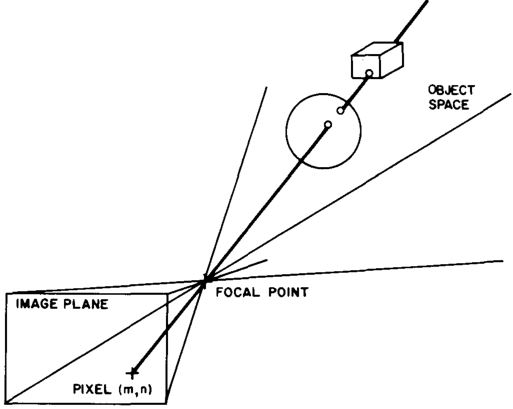
\includegraphics[width=0.47\linewidth]{whitted01}\hspace*{0.25cm}
        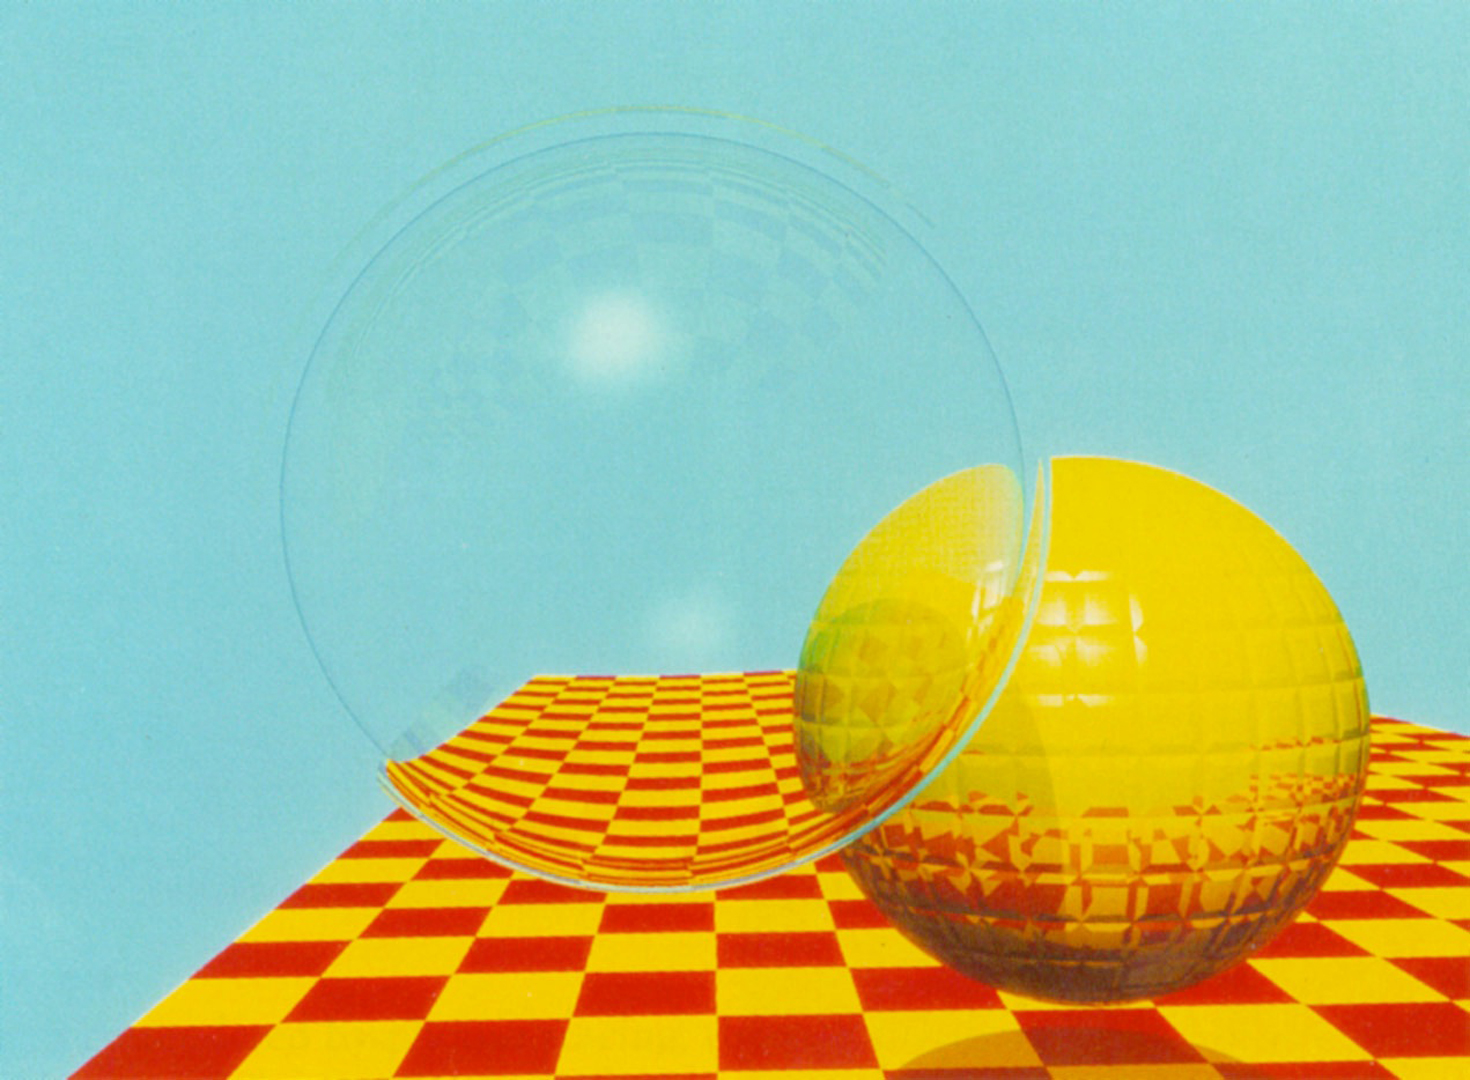
\includegraphics[width=0.775\linewidth]{whitted02}
        %\caption{Visualisierung eines Raytracing-Vorgangs \cite{Suffern}}
    \end{figure}
    
    %\vspace{120px}

	\begin{itemize}
		%\item Algorithmus der Computergrafik zum Rendern mit globaler Beleuchtung
	 	\item Standardthema in Vorlesungen der Computergrafik 
	 	%\item \textbf{Problem:} \\ Verständnis des Ablaufs durch reine Theorie oft nicht direkt ersichtlich
	 	\item Visualisieren des Prozesses in einer Virtual Reality Umgebung
	\end{itemize}

%\vspace{1cm}

\end{block}

%\vspace{0.125cm}

\end{column}

% -------

\begin{column}{.025\textwidth}\end{column} % Empty spacer column

\begin{column}{0.465\textwidth}

\begin{block}{Virtual Science Laboratories}
   \begin{figure}
       %\includegraphics[width=0.95\linewidth]{dxrWorkspace} %\textwidth]{dxrWorkspace}
   	  \includegraphics[height=14.25cm]{hmd}\hspace*{0.25cm}
       \includegraphics[height=14.25cm]{dxrWorkspace}
   	 % 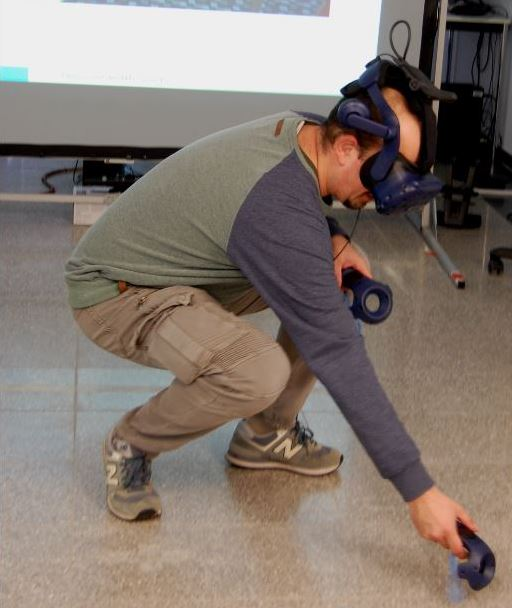
\includegraphics[height=14.25cm]{hmdSmall}
   	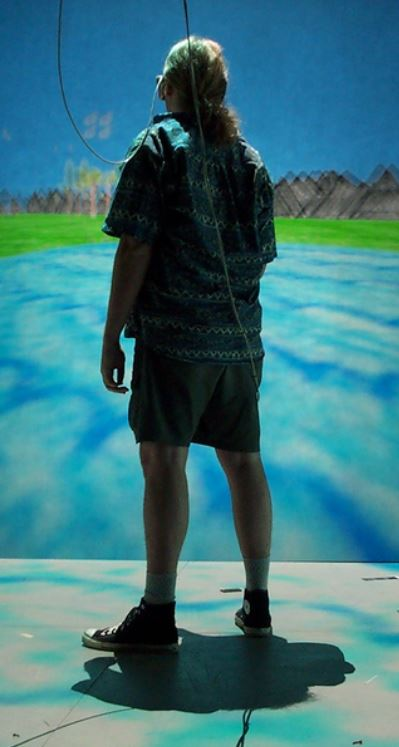
\includegraphics[height=14.25cm]{caveSlim}
   \end{figure}
   
   \begin{itemize}
   \item Unter dem Sammelbegriff \textbf{Cross-Reality (XR)} werden Techniken der digitalen Konstruktion und Unterst\"utzung von Realit\"aten zusammengefasst.
   \item Applikationen dieser Art finden vermehrt Einsatz in Industrie, Unterhaltung und Lehre.
   \item Im \textbf{Virtual Science Lab} der Hochschule Kaiserslautern werden Prototypen konzeptioniert und entwickelt, um die Lehre an der Hochschule besser unterst\"utzen zu k\"onnen.
   \end{itemize}
   
     
   
   
\end{block}


\end{column} % End of the second column



\begin{column}{.025\textwidth}\end{column} % Empty spacer column

\end{columns} % End of all the columns in the poster


%\vspace{0.125cm}

% ---

\begin{columns}[t] % The whole poster consists of two major columns, each of which can be subdivided further with another \begin{columns} block - the [t] argument aligns each column's content to the top

\begin{column}{.025\textwidth}\end{column} % Empty spacer column

\begin{column}{.96\textwidth} % The first column


\begin{block}{Visual Raytrace}

    \begin{figure}
        \centering
        
        \begin{subfigure}[b]{0.49\textwidth}
        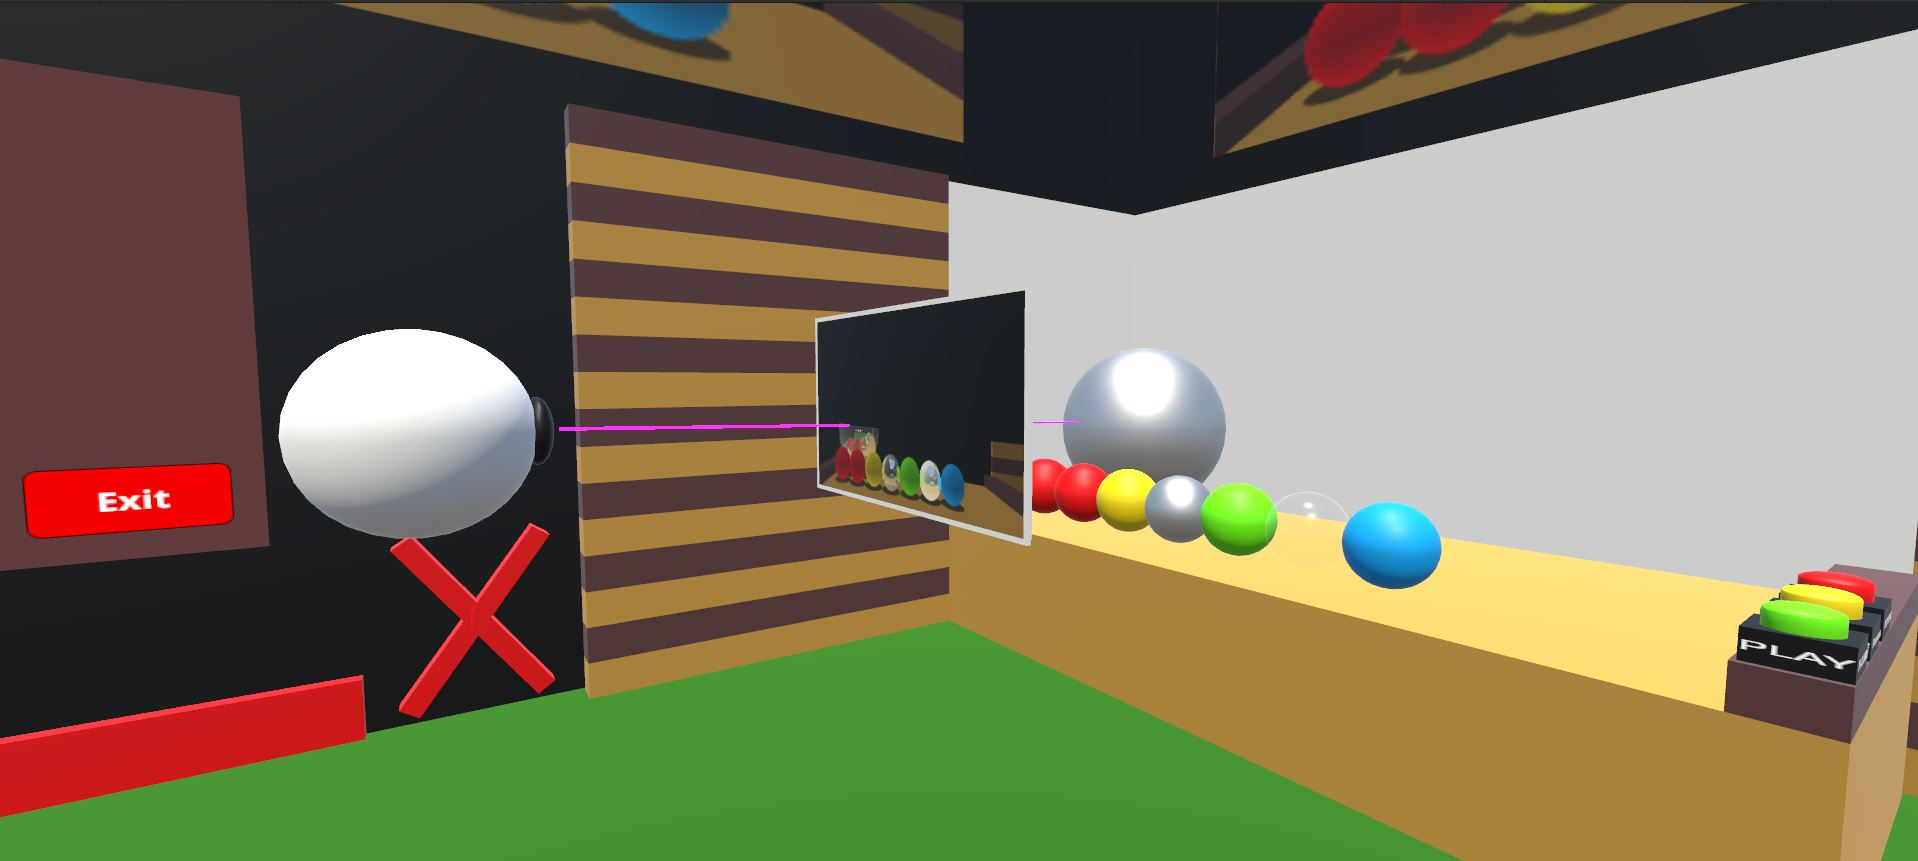
\includegraphics[width=\textwidth]{duringProcess}
        \end{subfigure}%
        \hfill%
        \begin{subfigure}[b]{0.49\textwidth}
        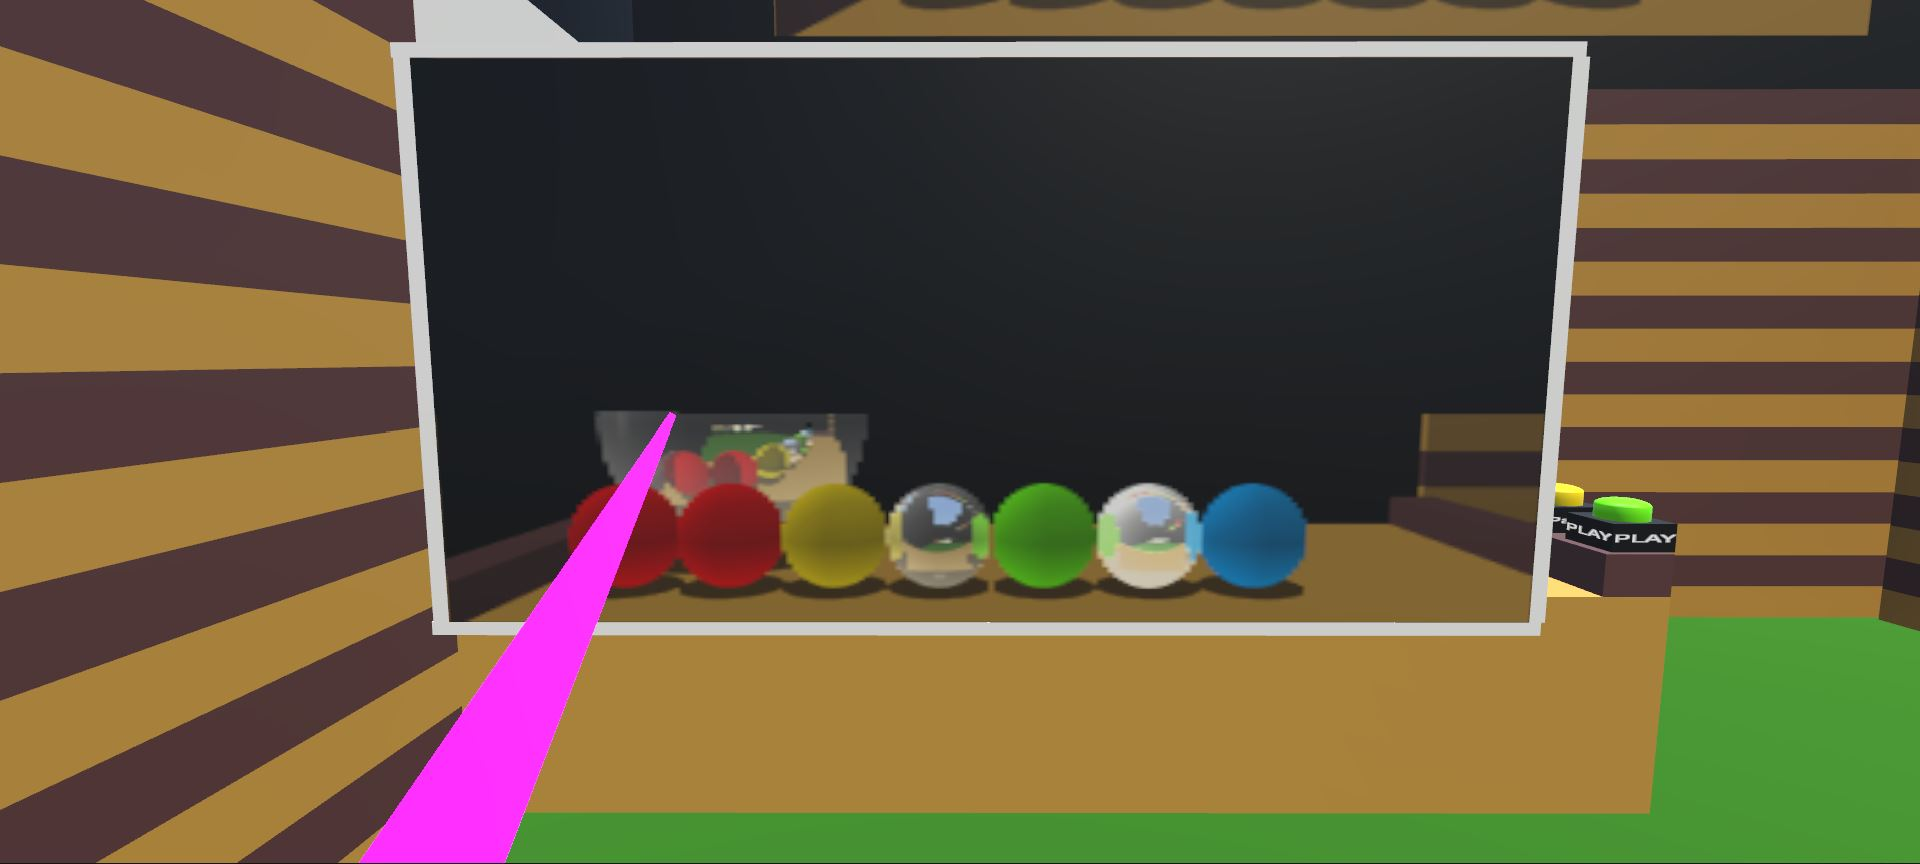
\includegraphics[width=\textwidth]{duringProcessEyeView}
        \end{subfigure}
       \end{figure}
       
     \vspace{1px}
	%\hfill
	
	\begin{figure}
	%\centering
        
        \begin{subfigure}[b]{0.49\textwidth}
        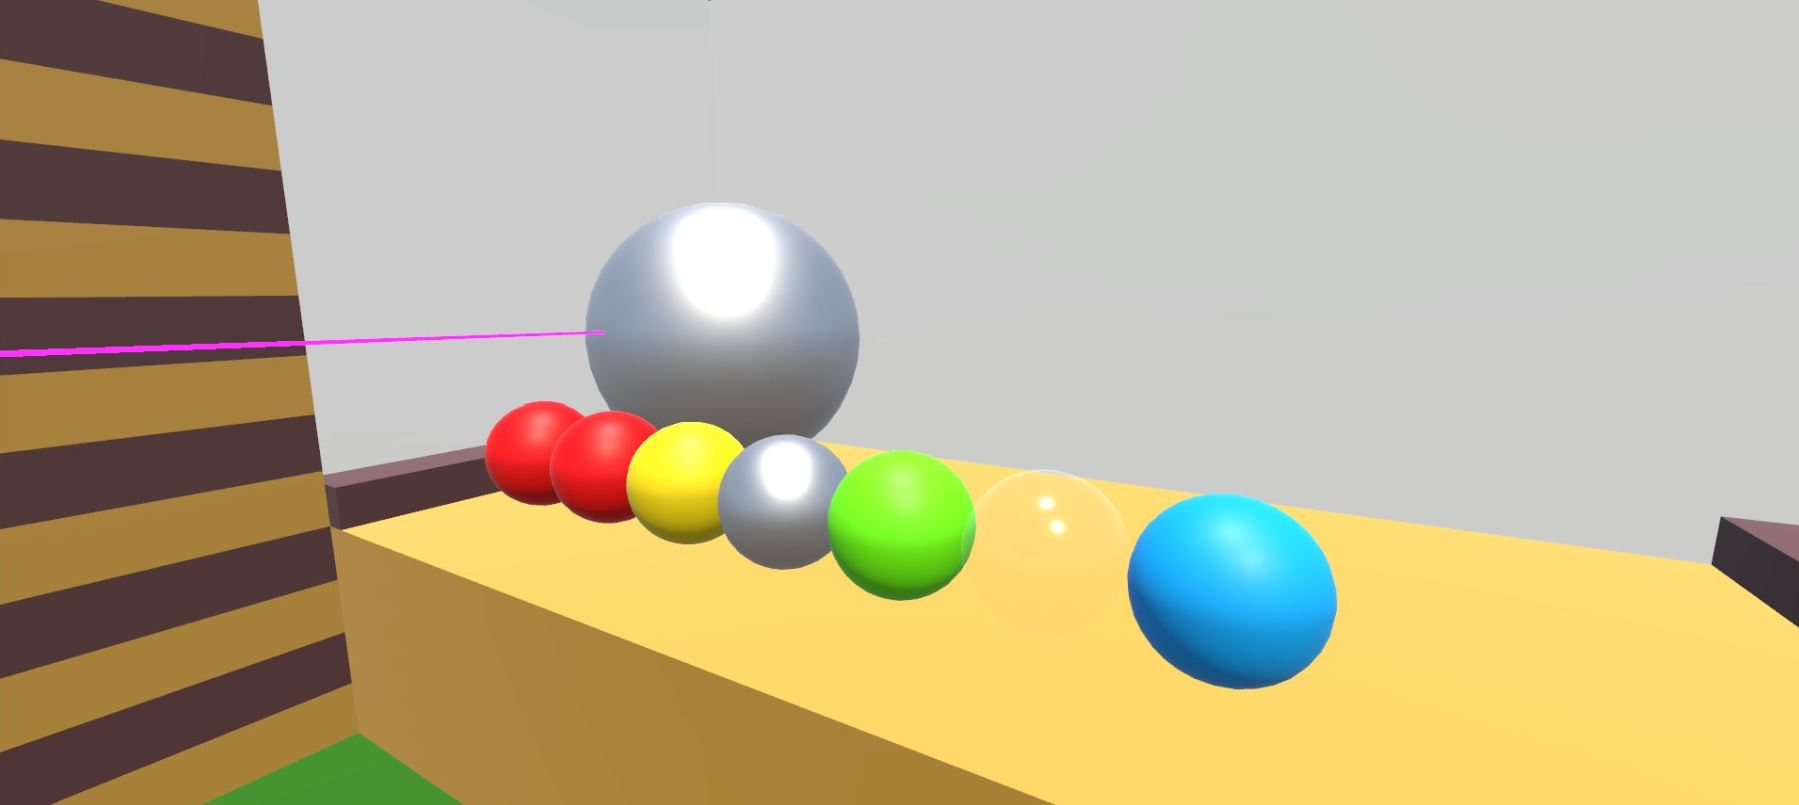
\includegraphics[width=\textwidth]{duringProcessHitObjects}
        \end{subfigure}%
        \hfill%
        \begin{subfigure}[b]{0.49\textwidth}
        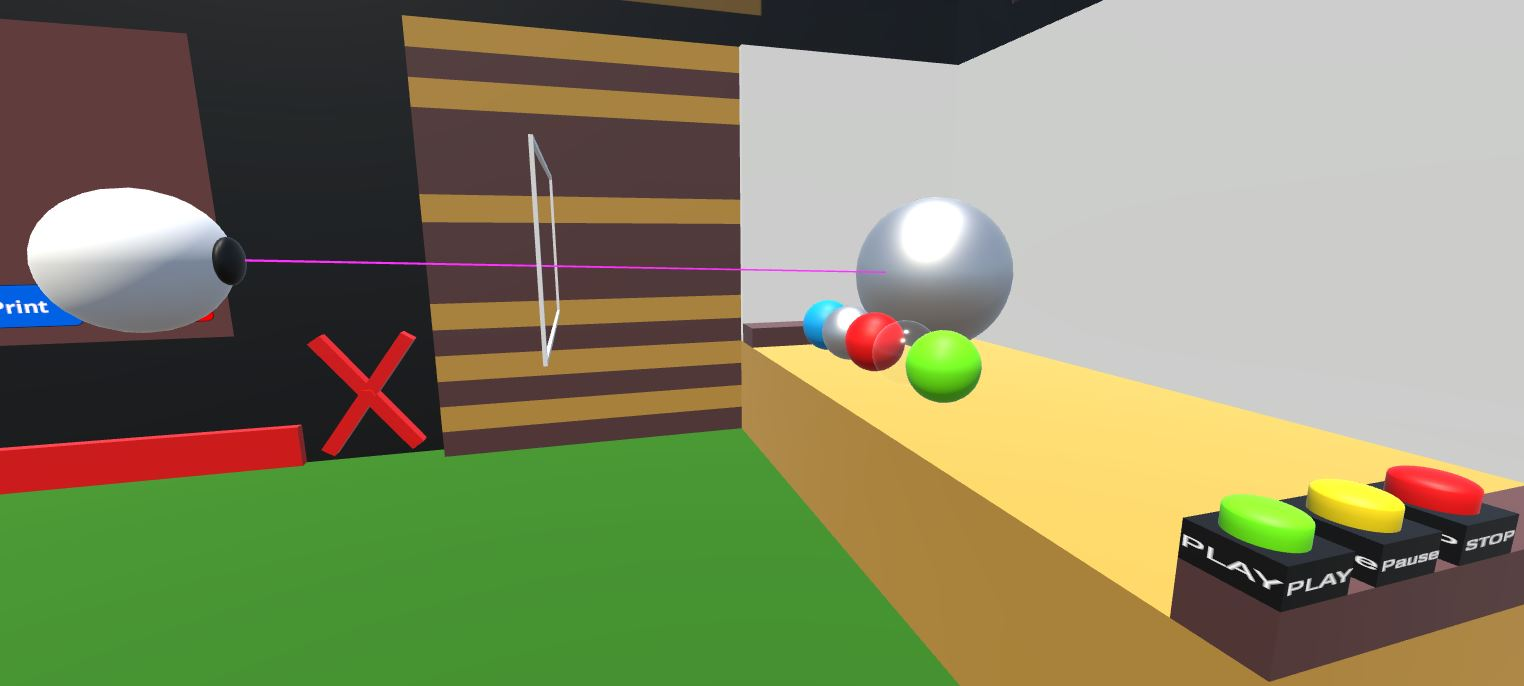
\includegraphics[width=\textwidth]{vorgang}            	   
    	\end{subfigure}
    
    \end{figure}

%\begin{itemize}
%	\item In der Applikation schie{\ss}t ein Auge mit Strahlen durch eine vordefinierte Ebene. Wird hinter der Ebene ein Objekt durch den Strahl erkannt, so wird basierend auf dem getroffenen Objekt eine Farbe berechnet. Die bestimmte Farbe wird dem aktuellen Pixel der Ebene zugeteilt, und der nächste Pixel wird mit einem neuen Strahl durchschossen.  
% \item Zielobjekte dieses Vorgangs sind Sphären. Die abgebildeten Sphären können durch simples Greifen in ihrer Position angepasst werden, um das finale Bild zu individualisieren. Weitere Sphären können jederzeit hinzugefügt werden. Zusätzlich kann jede Sphäre in ihrer Farbe und Material verändert werden, um z.B. Reflexionen zu simulieren.  
%  \item Der Benutzer kann den Raytracing-Prozess durch Betätigen von Buttons in der Szene steuern und verfolgen.
 
%\end{itemize}
    
    %\vspace{20px}
\end{block}

\end{column}

\begin{column}{.025\textwidth}\end{column} % Empty spacer column

\end{columns} % End of all the columns in the poster



\begin{columns}[t] % The whole poster consists of two major columns, each of which can be subdivided further with another \begin{columns} block - the [t] argument aligns each column's content to the top

\begin{column}{.025\textwidth}\end{column} % Empty spacer column

\begin{column}{.4675\textwidth} % The first column


\begin{block}{Materialien}
    %\vspace{140px}
    \begin{figure}
    	\center
        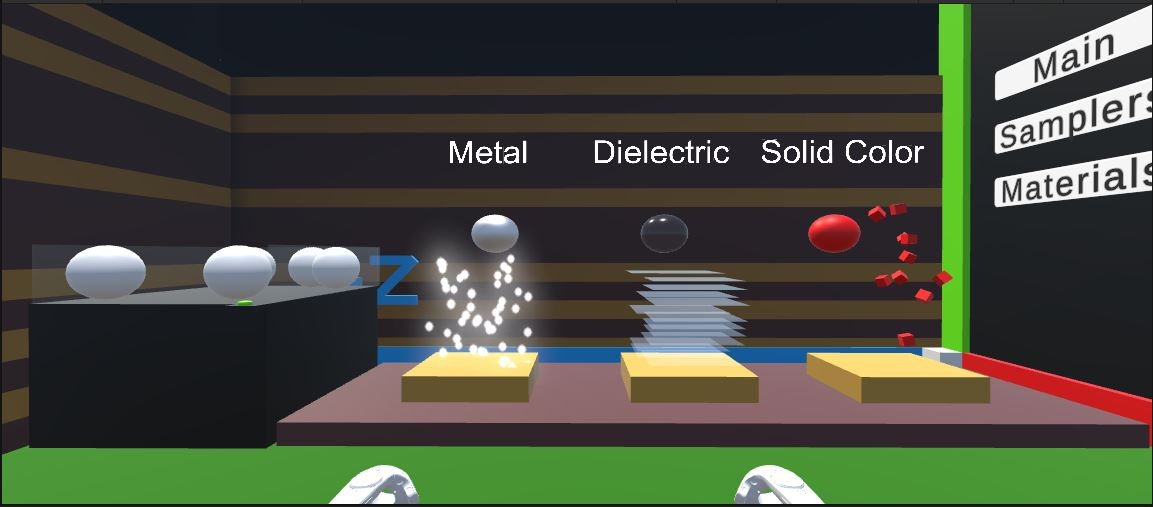
\includegraphics[height=16.5cm]{sphereCreating}
        %\hspace*{0.25cm}
        %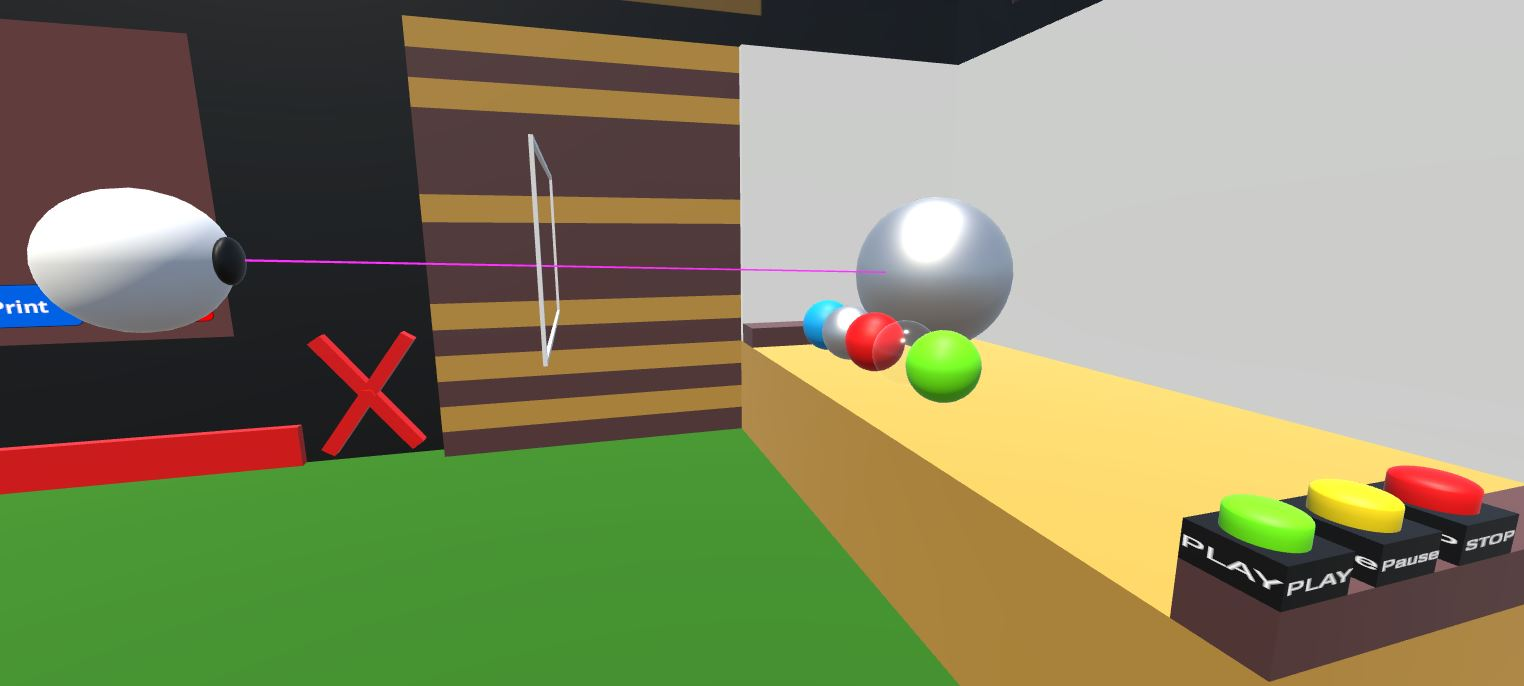
\includegraphics[width=0.45\textwidth]{vorgang}
        %\caption{Visualisierung eines Raytracing-Vorgangs \cite{Suffern}}
    \end{figure}

%\vspace{10px}

	%Jede Sphäre besitzt ein Oberflächenmaterial. Dieses Material definiert Eigenschaften wie Farbe und Lichtverhalten für ein Objekt. In der Applikation stehen 3 Materialien zur Auswahl:
    
    %\vspace{10px}

	\begin{itemize}
		\item Interaktive Vergabe von Oberflächenmaterialien
		%\item \textbf{SolidColor}: Einfarbiges Material für simple Farbsphären 
	 	%\item \textbf{Metal}: Reflektierendes Metall, in dem sich andere Objekte spiegeln 
	 	%\item \textbf{Dielectric}: Transparente Glassphären
	\end{itemize}

%\vspace{1.55cm}

\end{block}

%\vspace{0.1cm}

\end{column} % End of the second column



\begin{column}{.02\textwidth}\end{column} % Empty spacer column

\begin{column}{.465\textwidth}

\begin{block}{Einstellungen}
   \begin{figure}
       %\includegraphics[width=0.95\linewidth]{dxrWorkspace} %\textwidth]{dxrWorkspace}
   	  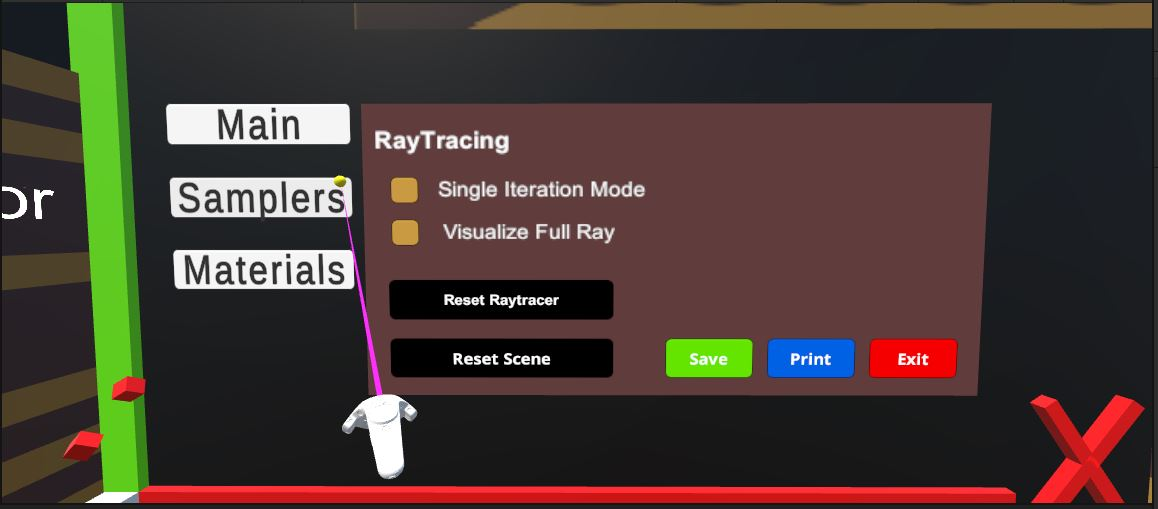
\includegraphics[height=16.5cm]{settings}
   	  %\hspace*{0.25cm}
       %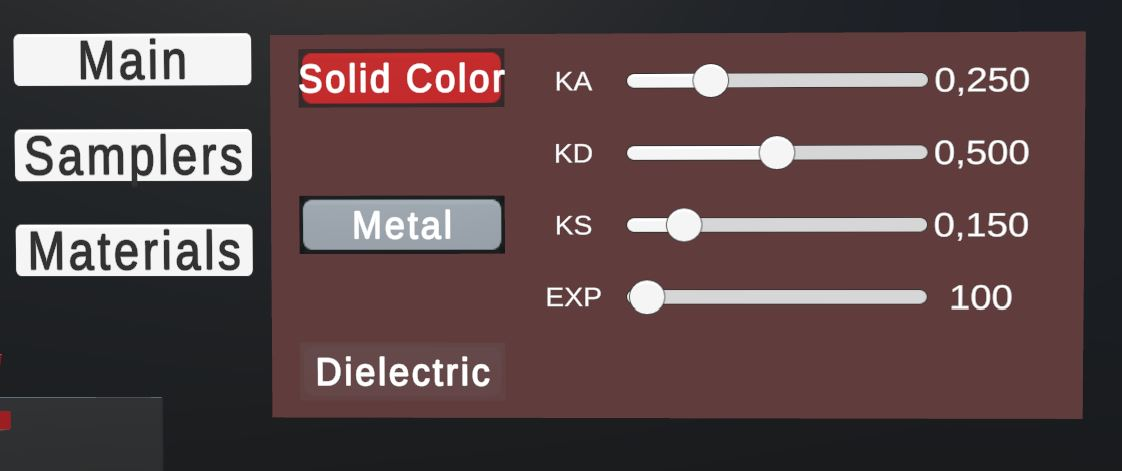
\includegraphics[width=0.49\textwidth]{settingsMaterials}%\hspace*{0.25cm}
       %\includegraphics[height=13.5cm]{hmd}
   	  %\includegraphics[height=13.5cm]{CAVE_Crayoland}
   \end{figure}
   
  % \vspace{10px}
   
   
   
   %Zur Steuerung des Raytracers existiert ein Einstellungsfenster in der Szene selbst. Mithilfe von Controllern können Elemente ausgewählt und angepasst werden.
   
   %\vspace{10px}
   
   \begin{itemize}
   \item Einstellungen für den integrierten Raytracer
   %\item Eigenschaften bzw. Parameter der Materialien anpassen
   %\item \textbf{Materials}: Eigenschaften bzw. Parameter der Materialen anpassen
   \end{itemize}
   
     
   
   
\end{block}


\end{column} % End of the second column



\begin{column}{.025\textwidth}\end{column} % Empty spacer column

\end{columns} % End of all the columns in the poster





%----------------------------------------------------------------------------------------

%\hrule





\begin{columns}

\begin{column}{0.02\textwidth}\end{column} % Empty spacer column

\begin{column}{0.15\textwidth}
\begin{figure}[h]
\centering
\includegraphics[scale=1.5, left]{qrCode}
\end{figure}
\end{column}

\begin{column}{0.01\textwidth}\end{column} % Empty spacer column

\begin{column}{0.325\textwidth}
\begin{itemize}
\item[] \textbf{\large Virtual Science Laboratories}
\item[] \faGlobe\ \href{https://webhome.hs-kl.de/~brill/}{https://webhome.hs-kl.de/~brill/} 
\item[] \Letter\ \href{benedict.saerota@hs-kl.de}{benedict.saerota@hs-kl.de}
\item[] \Letter\ \href{manfred.brill@hs-kl.de}{manfred.brill@hs-kl.de}
\item[]
\item[] \includegraphics[scale=0.475]{icon/githubIcon} \href{https://github.com/VRLAB-HSKL/RayTracing}{http://github.com/VRLAB-HSKL/RayTracing}

\end{itemize}
\end{column}

%\begin{column}{0.025\textwidth}\end{column} % Empty spacer column

\begin{column}{0.465\textwidth}
\nocite{*}
\begin{block}{Literatur}
 \bibliographystyle{geralpha}
 \nocite{pries:19}
 \bibliography{bib/sample}
\end{block}
\end{column}

\begin{column}{0.025\textwidth}\end{column} % Empty spacer column


\end{columns}

\end{frame} % End of the enclosing frame

\end{document} 